\setlength{\columnsep}{5pt}
\begin{flushleft}
	\paragraph{}
	\begin{itemize}
		\item A Linux distribution (or distro) is made from the \textbf{Linux kernel and collection of software}.
		\item Almost one thousand Linux distributions exist.
		\item Free and community managed distributions are:
		\begin{figure}[h!]
			\centering
			
\includegraphics[scale=0.4]{content/chapter1/images/distro.png}
			\caption{Linux distributions}
			\label{fig:distro1}
		\end{figure}
		
		\item Popular commercially backed distributions are:
		\begin{figure}[h!]
			\centering
			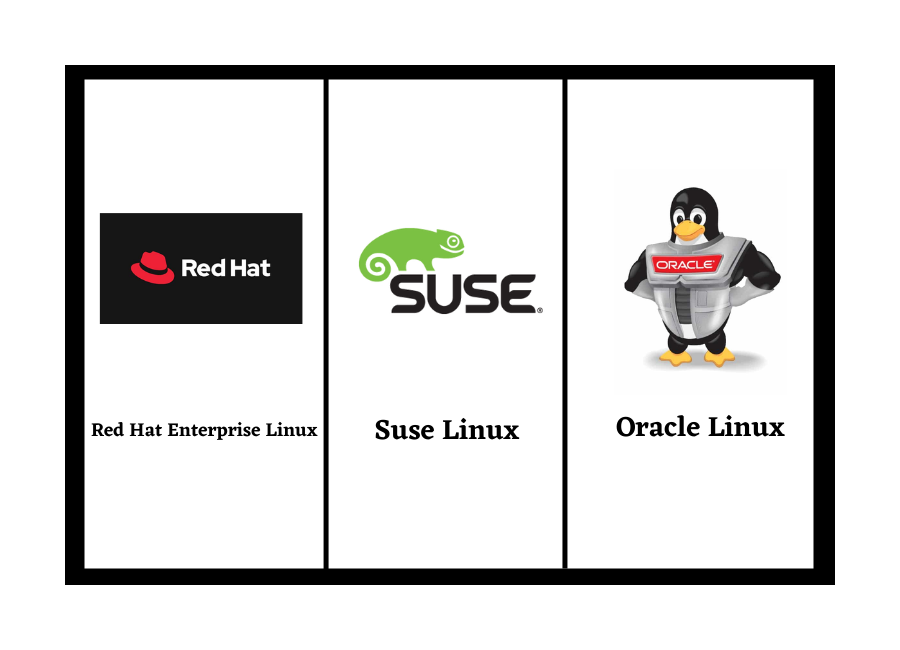
\includegraphics[scale=0.3]{content/chapter1/images/distro2.png}
			\caption{Commercial Linux distributions}
			\label{fig:distro2}
		\end{figure}

	\end{itemize}

	\newpage
	\paragraph{What is upstream and downstream?}
	\begin{itemize}
		\item The term 'upstream' refers to the \textbf{original version of a software}.
		\item Downstream is the \textbf{refined product code} based on original software version.
		\item Eg:
		\begin{itemize}
			\item \textbf{Fedora} is the upstream to \textbf{Red Hat Enterprise Linux (RHEL)}.
			\item \textbf{Debian} is the upstream to \textbf{Ubuntu}.
		\end{itemize}
	\end{itemize}
\end{flushleft}
\newpage
